%*************************************************************
% Master Project                                             *
% Ing. Minerva Gabriela Vargas Gleason                       *
% IAI - Institute of Artificial Intelligence                 *
% Universität Bremen                                         *
%                                                            *
% pdfLaTex                                                   *
% Editor: TeXnicCenter                                       *
%*************************************************************


\chapter{Background \&  Related Job}


This chapter presents the current state of the art of some relevant topics for mobile robotics that the reader needs to fully understand the content of this thesis. The first section will refer to mobile robots' localization.

\section{Localization Algorithms (\textit{if moving the base is required})}

Robot localization can be defined as the on-line estimation of a mobile robot's position based on sensor data; the position is given with respect to a global coordinate frame. Nowadays, localization is a fundamental research problem in robotics since it is required for most mobile robotics' tasks.

According to \citet{Markov}, the aim of \textit{localization} is to estimate the position of a robot, given a map of the environment and data from the robot's sensors. Localization is often referred to as \textit{position estimation}.

The current localization techniques can be separated on two groups according to the problem they solve (\citep{Markov}):
\begin{itemize}
	\item \textbf{Tracking or local:} In this case, the initial position of the robot is known and the algorithm only has to compensate for odometry errors that appear when the robot moves. The main problem they present is that they cannot recover if they lose track of the robot's position (considering some threshold).
	\item \textbf{Global:} These are able to obtain the initial position of a robot. In other words, they estimate the robot's position under global uncertainty. This is commonly known as the \textit{wake-up robot problem}, where the initial location of the robot is unknown.
\end{itemize}

A well-known problem in robot localization is known as the \textit{kidnapped robot problem}, where a robot is carried to a different location. Hence the robot must be able to determine whether the previous known position is wrong and,if it is, find its current location. Global algorithms are able to solve this problem. 

\subsection{Markov Localization (\textit{if required})}

The \textit{Markov Localization} is a global technique that estimates the position of the robot based on a probabilistic framework. Basically, what Markov localization does is represent the robot's belief by a probability distribution over possible positions \citep{Montecarlo}. The belief is updated using Bayes rule every time the robot moves or receives data from its sensors. 

Let us denote the robot's position by  $l=(x,y,\theta)$, where $x$ and $y$ are the robot's coordinates with respect to a fixed world reference frame, and $\theta$ is the robot's orientation. The probability distribution that states the robot's belief of being at a certain position $l$ is given by $Bel(l)$.

As shown in Figure \ref{fig:markov}, the robot starts with a uniform distribution of belief states representing that it is equally probable for the robot to be in any position in the environment. After receiving data from the sensors, the belief $Bel(l)$ is updated and the more probable positions obtain a higher value. Eventually, the robot becomes highly certain about its position, which is represented by a narrow Gaussian distribution centered around the robot's current location.

\begin{figure}[H]
	\centering
	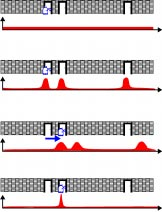
\includegraphics[width=0.4\linewidth]{markov.png}
	\vspace{-10pt}
	\caption{Markov localization: basic concept. \citep[chap. 2, page 393]{Markov}}
	\vspace{-15pt}
	\label{fig:markov}
\end{figure}

As explained by \citet{Montecarlo}, the belief is updated with two different probabilistic models: a model that represents the robot's motion and a perception model that considers the sensor readings:
\begin{itemize}
	\item \textbf{Robot motion:} The probability that a measured movement $a$ occurs at a certain position $l'$ is given by $P\ (l\ |\ l',\ a)$. This model is used to update the belief state every time a movement is executed.
	\begin{equation}
	Bel(l) \leftarrow \int P\ (l\ |\ l',\ a)\ Bel(\ l')\ dl' 
	\end{equation}
	\item \textbf{Sensor readings:} The probability of receiving a sensor reading $s$ when the robot is at the location $l$ is given by $P\ (s\ |\ l)$. We can use this to update the robot's belief with:
	\begin{equation}
	Bel(l) \leftarrow \alpha \ P\  (s \ |\ l \ )\ Bel(l)
	\end{equation}
	where $\alpha$ is a normalization factor that makes $Bel(l)$ integrate to 1.
\end{itemize}

Markov localization is able to globally estimate the position of the robot, recover from uncertainties and odometry errors and solve the kidnapped robot problem (re-localize the robot). 

This localization technique uses a probability distribution over the space of all hypotheses of where the robot can be ($Bel(l)$) to estimate the current robot location. The computational resources needed to maintain this probability distribution for all possible positions increase with the size of the space. For normal environments, the required memory can easily exceed 100MB. The problem with the high computational cost also appears in \textit{grid-based} Markov localization approaches, which discretize the relevant parts of the space using an evenly spaced grid of points.

This technique works under the assumption that the environment is static (\textit{Markov assumption}), which is not true in some applications of mobile robotics. Sometimes, the robot can be located in an environment where it interacts with people and objects that can be moved. To solve the localization problem in this case, a different technique is required.

\subsection{Monte Carlo Localization (\textit{if required})}

Monte Carlo Localization (MCL) is a version of sampling-importance-resampling (SIR) based on Markov localization. It is a sample-based algorithm that uses particle filters to ensure the survival of the fittest.

According to \citet{Montecarlo}, this algorithm uses fast sampling techniques to represent the robot's belief $Bel(l)$ by estimating the posterior distribution every time the robot moves or senses using the importance re-sampling technique.

MCL uses many samples during the global localization and the sample set size is significantly reduced during tracking when an approximate position of the robot is already known. Compared to grid-based Markov localization, MCL requires considerably less memory and, therefore, can integrate measurements at a higher frequency. It is more accurate and easier to implement than Markov localization. The main advantage MCL has is that it is able to perform \textit{global localization}, meaning that MCL can obtain the initial position of a robot and solve the \textit{kidnapped robot problem} at a low computational cost. This allows us to use MCL in bigger environments.

The key concept of this approach is to represent the posterior belief $Bel(l)$ by a set of $N$ weighted, random particles $S=\lbrace s_i\  \vert \ i=1...\ N\rbrace$. This sample set is a discrete approximation of a probability distribution. The distribution is updated by updating the weight of each particle after every sensor's reading or robot's movement.

The samples are represented by $\langle\langle x,\ y,\ \theta\rangle,\ p\rangle$, where the first three parameters denote a possible robot position  and $p$ is the weighting factor of the particle ($p\geq\ 0$). Assume $\sum_{n=1}^{N} p_n\ = 1$, all weights must be normalized so that they sum up to 1.

As explained by \citet{Montecarlo}, updating the particle set is done in two different ways:
\begin{itemize}
	\item \textbf{Robot Motion:} Every time the robot moves, $N$ new samples are randomly created. These new samples approximate the robot's position with respect to the motion command. Each new sample is generated from the previous sample set with it's likelihood determined by the particle's weight. The location of the new sample is given by:
	\begin{equation}
	\vspace{-20pt}
		P\ (l\ \vert l'\ ,\ a)
	\end{equation}
	where $a$ is the observed movement and $l'$ the previous location. Figure \ref{fig:motion} shows the behavior of this sampling technique where the robot starts with a known position and moves following the straight lines.
	
	The uncertainty of the sample sets increases with each iteration. This uncertainty represents the error in the robot's location due to slippage and drift.
	\item \textbf{Sensor readings:} The sample set is re-weighted implementing Bayes' rule. For a sample $\langle\ l,\ p\ \rangle$, the update rule is:
	\begin{equation}
	\vspace{-20pt}
	p \leftarrow \alpha \ P\  (s \ |\ l \ )
	\end{equation}
	where $s$ is the sensor information and $\alpha$ a normalization factor that ensures the weights satisfy $\sum_{n=1}^{N} p_n\ = 1$.
\end{itemize}

\begin{figure}[H]
		\centering
		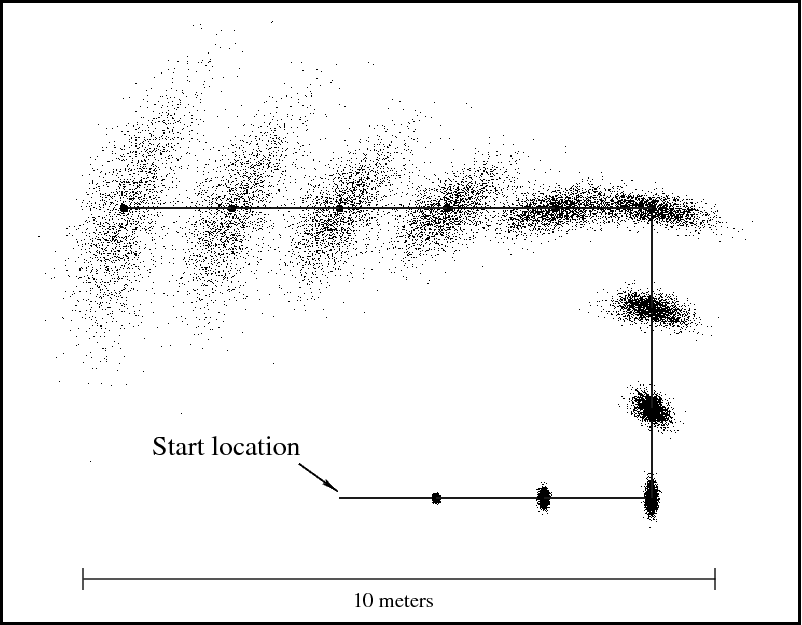
\includegraphics[width=0.5\linewidth]{robot_location.png}
		\vspace{-10pt}
		\caption{ MCL approximation of the position's belief based only on motion commands 			\citep[page 3]{Montecarlo}.}
		\vspace{-15pt}
		\label{fig:motion}
\end{figure}

In every iteration, the sample set is centered around the robot's believed position, in case of an error in location (such as in the \textit{kidnapped robot problem}, the robot wouldn't be able to re-localize itself. In order to avoid this problem, after each update some random, uniformly distributed samples are added to the set. These added samples are used in case the robot loses track of its position. The random samples uniformly distributed in the whole environment can effectively re-localize the robot. In case the position of the robot is not lost, the weight of these random samples will decrease and the samples will disappear in the next iteration.

\begin{figure}[H]
	\centering
	\begin{subfigure}[][Initialization]
		{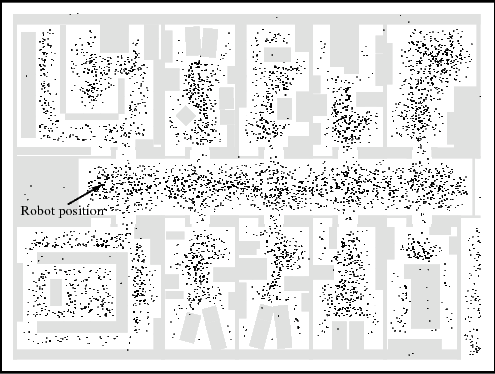
\includegraphics[width=0.32\linewidth]{position1.png}}
	\end{subfigure}
	\begin{subfigure}[][Uncertainty due to symmetry]
		{\label{subfig:goal}
		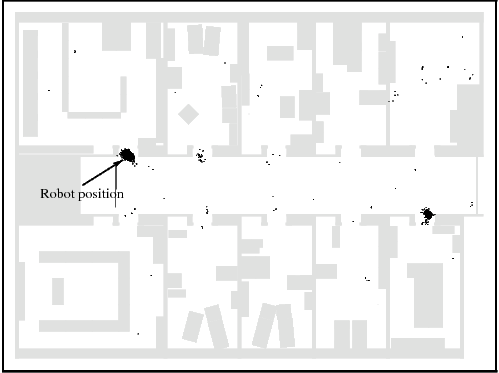
\includegraphics[width=0.32\linewidth]{position2.png}}
	\end{subfigure}
	\begin{subfigure}[][Final localization]
		{\label{subfig:goal}
		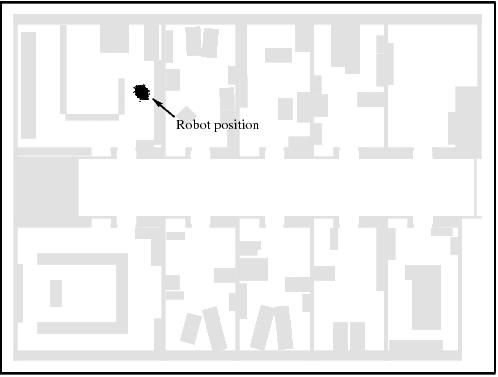
\includegraphics[width=0.32\linewidth]{position3.png}}
	\end{subfigure}
	\vspace{-12pt}
	\caption{Global localization of a robot using MCL}
	\vspace{-15pt}
	\label{fig:example}
\end{figure}
\vspace{-8pt}

Figure \ref{fig:example} shows an example of a global localization performed by a robot using MCL. The first image shows the initial sample set distribution where the robot's position is unknown and the samples are uniformly distributed throughout the environment. The second image shows two probable robot positions after the robot has slightly moved; this uncertainty is caused by a symmetry in the map. The random samples in the second image are the ones added after each update. The third image shows the successful localization of the robot after it kept going forward. The information used to achieve this localization was the movement commands and the sensor information.

Nowadays, there are several programs that provide localization capabilities using simultaneous localization and mapping (SLAM). SLAM is the process of constructing a map of an unknown environment while keeping track of the agent's location in it. The agent is normally a robot or an autonomous vehicle.

In the next section, a new SLAM software will be presented: \textit{Google Cartographer}. Google cartographer can obtain information from two different types of sensors, namely sonar and laser scanners, and can be implemented in virtually any mobile robot.

\section{Kinematic Modelling of a Robot}

According to \citet{Handbook}, \textit{robot kinematics} refers to the motion of the elements in a robot without considering the forces and torques that generated this movement. 
To describe the movement of a robot, we need a kinematic model of its structure. The position and orientation of a body  in space is known as \textit{pose}.

A robot can be modelled as a kinematic chain, which consists of a system of rigid bodies connected by joints, a \textit{kinematic joint} is a connection between 2 bodies that constrains their relative motion. These bodies are called \textit{links}.  The kinematic description of a robot normally uses some simplifications: the links that form the robot are assumed to be rigid, and each link is ideally connected with the next one, with no gap in between.
\begin{figure}[H]
	\centering
	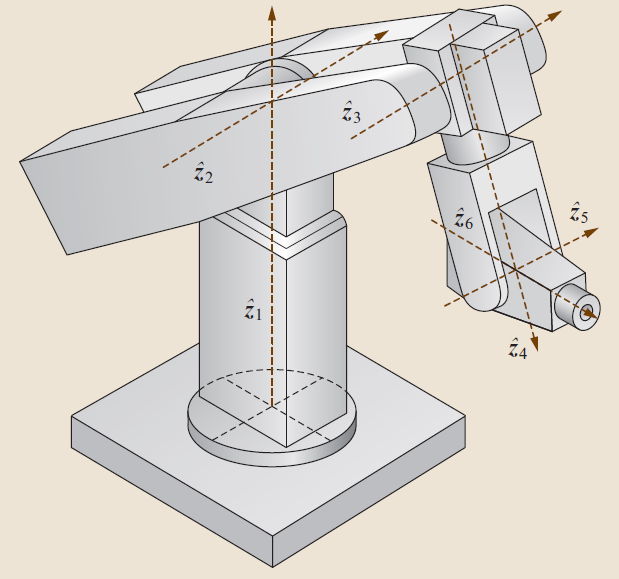
\includegraphics[width=0.5\linewidth, angle=0]{6dof-robot.png}
	\vspace{-10pt}
	\caption{Example of a 6 DOF manipulator. \citep[chap. 1, page 24]{Handbook}}
	\vspace{-15pt}
	\label{fig:kinematic}
\end{figure}

Figure \ref{fig:kinematic} shows an example of a serial chain manipulator, where a reference frame is attached to each link. Following the Denavit-Hartenberg convention, the \textit{Z} axis is always aligned with the joint axis \citep{Craig}.

The study of robot kinematics involve how the location of the reference frames change as the mechanism moves. The main goal is to compute the position and orientation of the manipulator's end-effector with respect to the base as a function of the joints values.

For an open-loop robotic mechanism, the general structure is represented by a kinematic tree, which consists of the concatenation of links and joints with a reference frame in each joint \citep{Handbook}. This representation is used to obtain a mathematical model of the system. 

When programming a robot, a suitable representation of its kinematic model is required. The Unified Robot Description Format (URDF) is a standard XML representation of the robot model in the ROS community\footnote{http://wiki.ros.org/urdf}, which includes the robot kinematics, dynamics, and sensors. In this project, I represented the model of Boxy with a URDF. A section of the kinematic tree of Boxy is found in Appendix \ref{A1}, it shows the neck (UR3) description.

\section{Collision Environment}

The workspace of a robot is defined as the total volume swept out be the end-effector as the manipulator executes all possible motions \citep[chap. 1]{Handbook}. In simple terms, the workspace is the space that can be reached by the robot.

The working environment consists of all the external factors surrounding and affecting the robot. In other words, it is the space where the robot is working, including all the objects in there. According to \citet{Taskspace}, the robot is considered to be operating in a "world" that it cannot leave; actions can affect the environment and, thus, change it for the robot. 

The environment can be represented in a graphical way with meshes that describe the geometry of the objects and of the robot. The position of the meshes in the model environment has to match the position of the real objects. Motion planning algorithms are then used to calculate trajectories that the robot can execute without colliding with the environment or itself. 

A robot can have two types of sensors \citep[chap. 1]{Russel}:
\begin{itemize}
	\item \textbf{Proprioceptive sensors:} Get information about the internal state of the robot, such as the angular position of each joint or the temperature of the links. These sensors are used for self maintenance and control of internal status. Examples of proprioceptive sensors are: shaft encoders, inertial navigation systems and force sensors.
	\item \textbf{Exteroceptive sensors:} Obtain information from the robot's environment, such as the distance to an object relative to a frame of reference of the robot. Many exteroceptive sensors are sensors that can be used to calculate distances. These sensors can be further categorized in contact, range, and vision sensors.
\end{itemize}

The robot takes the information from proprioceptive sensors to calculate the position and orientation of each link and determine its current configuration, and the information from exteroceptive sensors to calculate its position relative to the environment and the distance to surrounding objects. Combining both, the motion planning algorithms can iterate until a collision-free path between the initial and desired position is found.

\section{Pinhole Camera Model}

Robots can use cameras as sensors to determine the relative position of objects with respect to the robot. The image obtained by the camera can be used to obtain 3-dimensional properties of objects from the location of the 2D image points \citep{Camera}. In order to do this, a 2D-3D mapping between the camera and a world reference frame is needed, this mapping is computed using a geometric camera calibration.
\begin{figure}[H]
	\centering
	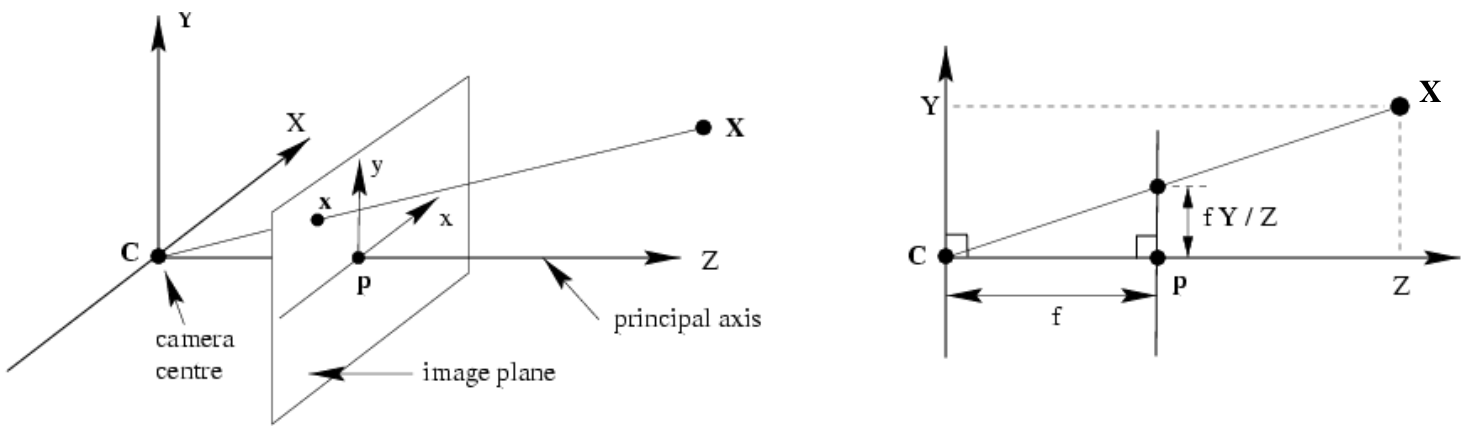
\includegraphics[width=0.9\linewidth, angle=0]{pinhole.png}
	\vspace{-10pt}
	\caption{Pinhole model of a camera.}
	\vspace{-15pt}
	\label{fig:pinhole}
\end{figure}

A simple model of a camera is the pinhole model, shown in  figure \ref{fig:pinhole}. The light in front of the camera converges at the pinhole and is projected onto the image plane inside the camera. A perfect lens could be modelled as a pinhole; however, all lenses cause some distortion, so the camera calibration should compensate the lens distortion. 

The equation describing this model is:
\begin{equation}
\mathbf{x}= \mathbf{PX}
\end{equation}
\begin{equation}
\left( \begin{array}{c}
X \\
Y \\
Z \\
1
\end{array}
\right)	\mapsto 
\left( \begin{array}{c}
fX + Zp_{x} \\
fY + Zp_{y} \\
Z
\end{array}
\right) = \left[ \begin{array}{cccc}
f & 0 & p_{x} & 0 \\
0 & f & p_{y} & 0 \\
0 & 0 & 1 & 0 \\
\end{array}
\right] \left( \begin{array}{c}
X \\
Y \\
Z \\
1
\end{array}
\right)
\label{eq:pin_camera}
\end{equation}
where $( p_{x}, p_{y})^T$ are the image principal point coordinates (offset between the corner of the image and the image center), \textit{f} is the focal length and \textit{X, Y, Z} are the coordinates of the object.

From \ref{eq:pin_camera}, we can obtain the camera calibration matrix:
\begin{equation}
\mathbf{K}= \left[ \begin{array}{cccc}
f & 0 & p_{x} & 0 \\
0 & f & p_{y} & 0 \\
0 & 0 & 1 & 0 \\
\end{array}
\right]
\label{eq:camera_calib}
\end{equation}

For this project, the pinhole model is a sufficient approximation, because the goal is only to center an object in the image. Since no precise 2D-3D mapping is required, the lens distortions doesn't affect the model. To position the camera, the normal vector of the camera lens has to point to the object. The robot must move the camera from the initial position to the goal position without colliding with any objects. 

The solution proposed in this project is currently configured for working only with one camera (it can be a stereo camera). If the number of sensors increases, the approach has to be modified, since the algorithm would not be able to decide which sensor to move. The current approach could work for several sensors if the user specifies which sensor has to arrive to the desired pose.

With the pinhole model, one can calculate the minimum and maximum distance required between an object and the camera. These distances depends on the size of the object and the field of view of the camera. In this project, we did not need to obtain these distances because the camera is always positioned between 1 and 2 meters away from the objects the robot is using, so the objects always fit in the camera's view. 

As future work, we propose to use the pinhole camera model to find useful distance ranges between the object and the camera, taking into account the size of the object.

\section{Trajectory Planning}

According to \citet[chap. 1, page 6]{trajectory} \textit{"A trajectory is the path that a moving object follows through space as a function of time"}. A trajectory can be described as a time-stamped series of location points.

To define a robot's trajectory, we must define the trajectory that each link will do to bring the robot to the desired pose.

Once the robot's kinematic model and environment are defined, we use a motion planning algorithm to solve the path planning problem and obtain a collision-free trajectory for the robot. The planning involves determining the path and the velocity function for a robot. 

\subsection{Euclidean Space in Cartesian Coordinates}

In geometry, we can describe the position of any object in space using Cartesian coordinates (X, Y, and Z). For a 3-dimensional space (Euclidean space), any object can move and rotate along 3 axes, this means that the object has 6 DOF, so 6 values are required to define the pose of an object with respect to a reference point. In other words, for a three-dimensional Euclidean space, we can describe the position and orientation of any object using the Cartesian coordinates and three rotation angles.

\subsection{Configuration Space (C-space)}
\label{subsec:cspace}

A complete description of the robot's geometry and of the workspace is needed to solve the path planning problem. A \textit{configuration} $\bm{q}$ specifies the location of every point of the robot's geometry. 

The \textit{configuration space}, where \( \bm{q} \in  \bm{C} \), is the space of all possible configurations \citep{Handbook}. It represents all possible transformations that can be applied to the robot given its kinematics. The C-space gives an abstract way of solving the planning, the main advantage is that a robot can be mapped into the C-space as a single point, where the number of DOF of the robot is the dimension of the C-space. This is also the minimum number of parameters required to describe a configuration, so motion planning for the robot is equivalent to motion planning for the C-space.

During trajectory planning, one must consider several constraints involving the robot's pose. Since the allowed configurations of the robot are not known beforehand, the planning algorithm must find these valid configurations while planning. Finding these configurations is normally done through sampling, this process can become inefficient for complex environments.

%\subsection{Task Space}

%According to \citet{Taskspace}, the \textit{task space representation} (TSR) are general representations of pose constraints that can be efficiently sampled for collision evaluation. TSRs can be chained to describe constraints of articulated objects, like a robot. These representation allows handling complex pose constraints using sampling algorithms for trajectory planning. 

\subsection{Motion Planning Algorithms}

As explained by \citet{Handbook}, the general path planning problem is computing a continuous free path for the robot between $\bm{q_{1}}$ and $\bm{q_{G}}$, given:
\begin{enumerate}
	\vspace{-5pt}
	\item The robot's workspace $\bm{W}$
	\vspace{-5pt}
	\item An obstacle region $\bm{O} \subset \bm{W}$
	\vspace{-5pt}
	\item A robot defined as a collection of \textit{m} links: $A_{1}, A_{2}, ... , A_{m}$
	\vspace{-5pt}
	\item The C-space $\bm{C}$ with defined $\bm{C_{obs}}$ and $\bm{C_{free}}$
	\vspace{-5pt} 
	\item An initial configuration $\bm{q_{1}} \in  \bm{C_{free}}$
	\vspace{-5pt} 
	\item A goal configuration $\bm{q_{G}} \in  \bm{C_{free}}$
\end{enumerate}

Where $\bm{C_{obs}}$ is the \textit{C-space obstacle region} and $\bm{C_{free}}$ is the set of configurations that avoid collision, called \textit{free space}. We must compute a continuous free path for the robot between $\bm{q_{1}}$ and $\bm{q_{G}}$.

The main complication is calculating $\bm{C_{obs}}$ and $\bm{C_{free}}$, that are needed to determine the region where the robot can move without colliding. There are two main approaches to solve the planning problem: sampling-based and combinatorial motion planning.

In this project, we will focus on sampling-based planners, since these are I decided to use in MoveIt! (section \ref{subsec:moveit}), our trajectory planning software.

\subsubsection{Sampling-based motion planning}
\label{subsec:planning}

The planner samples different configurations in the C-space to construct collision-free paths. These paths are stored as 1D C-space curves. The main idea is to avoid the direct construction of the obstacle region $\bm{C_{obs}}$. This means that instead of considering the obstacles directly, the planner uses a collision detector for each pose in the trajectory. This approach allows using the planner for a wide range of applications, we must only adapt the collision detector to the geometry of a specific robot.
\begin{figure}[H]
	\centering
	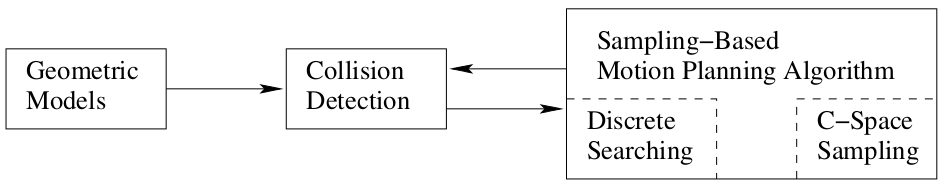
\includegraphics[width=0.9\linewidth]{sampling_alg.png}
	\vspace{-10pt}
	\caption{Sampling-based planning philosophy \citep[chap. 5, page 185]{planning}.}
	\vspace{-15pt}
	\label{fig:sampling}
\end{figure}

The sampling-based planning, shown in figure \ref{fig:sampling}, uses the collision detection as a "black box" between the motion planning and the geometric model of the robot. This generates an algorithm that is independent of the robot's geometry \citep{planning} .

This "black box" approach can solve problems that involve thousands of geometric primitives representing the robot. It is practically impossible, according to \citet{Handbook}, to solve such problems with algorithms that uses the $\bm{C_{obs}}$ directly.

The disadvantage of these algorithms is that they don't assure to find a solution in a finite amount of time. Combinatorial motion planning algorithms are able to return a solution, if it exists, in a finite amount of time.

A \textbf{rapidly exploring random tree (RRT)} is a sampling-based planning algorithm that searches a collision-free path by randomly building a space-filling tree. It has a good performance and does not require any parameter tuning. As shown in figure \ref{fig:rrt}, RRT reaches unexplored regions after just a few iterations. 
\begin{figure}[H]
	\centering
	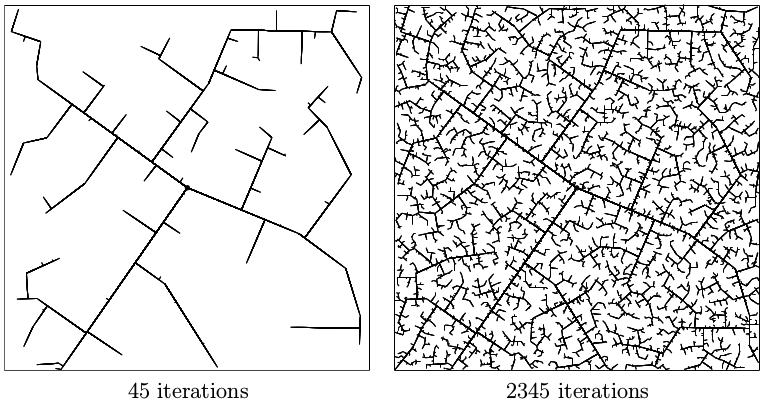
\includegraphics[width=0.7\linewidth]{rrt.png}
	\vspace{-10pt}
	\caption{Rapidly exploring random tree \citep[chap. 5, page 230]{planning}.}
	\vspace{-15pt}
	\label{fig:rrt}
\end{figure}
The basic idea of RRT is to incrementally build a search tree in the C-space that tries to connect $\bm{q_{1}}$ and $\bm{q_{G}}$, avoiding the obstacles in the way, where $\bm{G}$ is the search graph. All the vertices of $\bm{G}$ are collision-free configurations. 

The steps of this RRT algorithm for a C-space with no obstacles are shown in Algorithm \ref{algor:rrt_alg} \citep{planning}. Let $\bm{S}\subset \bm{C_{free}}$ be the set of all points reached by $\bm{G}$. Each iteration, a new vertex is created and connected to the closest point in $S$ along the shortest possible path. 

If there are obstacles, the tree will go up to the obstacle's boundary, approaching as close as the collision detection algorithm allows.

\begin{algorithm}[t!]
	\caption{Basic RRT}\label{algor:rrt_alg}
	\begin{algorithmic}[1]
		\State $\bm{G}.init(q_{1})$;
		\For{$i=1$ to $K$} 
		\vspace{-2pt}
		\State $\bm{G}.add\_vertex(\alpha(i))$;
		\vspace{-2pt}
		\State $q_n \longleftarrow$ NEAREST$(S(\bm{G},\alpha(i))$;
		\vspace{-2pt}
		\State $\bm{G}.add\_edge(q_n,\alpha(i))$;
		\vspace{-2pt}
		\EndFor 
	\end{algorithmic}
\end{algorithm}

The planner uses the obtained trees to find a path in $\bm{C_{free}}$ between the initial and the desired configuration. There are two different approaches for finding this path (figure \ref{fig:rrt_ex}):
\begin{itemize}
	\item \textbf{Single-tree search:} The planner grows a tree from $\bm{q_1}$ as shown in figure \ref{fig:rrt} and checks in every step if it is possible to reach $\bm{q_G}$ with the $\bm{S}$ created by the tree.
	\item \textbf{Balanced, bidirectional search:} Instead of creating only one RRT, it creates an aditional tree that starts from $\bm{q_G}$, this is quite effective when obstacles are partially surrounding $\bm{q_G}$ or $\bm{q_1}$. The graph $\bm{G}$ is formed by two trees, $T_a$ and $T_b$, growing from $\bm{q_1}$ and $\bm{q_G}$ respectively. Here, $\bm{S}$ is formed by $T_a$ and $T_b$. After some iterations, the trees are swapped, so $T_b$ is now growing around $\bm{q_1}$. Then, $T_b$ connects to a new vertex created for $T_a$, this causes that $T_b$ tries to grow towards $T_a$ and vice-versa. The solution is found when both trees connect.
\end{itemize}

\begin{figure}[H]
	\centering
	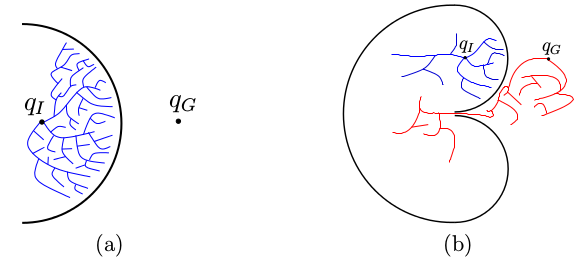
\includegraphics[width=0.7\linewidth]{rrt_example.png}
	\vspace{-10pt}
	\caption{ a) Single tree RRT, b) Bidirectional RRT \citep[chap.5, page 219]{planning}.}
	\vspace{-15pt}
	\label{fig:rrt_ex}
\end{figure}

The bidirectional search gives much better performance compared to the single-tree search.

\subsubsection{Optimization-based motion planning}

Sample-based VS Optimization-based

\section{Software}
In the last years, the number of applications where humans and robots work in proximity to each other has increased. This has lead to the development of many software programs used for robot manipulation. 

The IAI uses ROS to communicate with the robots, so this project was done using ROS as the base. ROS communicates the UR3, which holds the Microsoft Kinect, with Boxy. For trajectory planning, I used MoveIt!, with RVIZ as a side tool for visualization.

\subsection{ROS}

\textit{Robot Operating System (ROS)} is an open source software that helps developers to create robot applications. According to the official documentation\footnote{\url{http://wiki.ros.org/ROS/Introduction}}, ROS is a meta-operating system, a system that handles other operating systems, it handles hardware abstraction, low-level device control, implementation of commonly-used functionality, message-passing between processes, and package management. ROS also provides a wide range of libraries and tools for robots, such as drivers and visualizers. Some of these libraries are focused on mobility, manipulation and perception tasks.

One of the ROS main components is its communication infrastructure. This has a message passing interface that provides inter-process communication and is seen as a middleware\footnote{\url{http://www.ros.org/core-components/}}. 

The communication consists of a publish/subscribe message passing system, where one program publishes information under a certain topic. All other programs subscribed to this topic will receive the information. A program can be sending information through one or more topics and, at the same time, receiving information from other topics. ROS works as the middleware that manages and distributes these messages.

ROS uses \textit{nodes} to do computations. A node is a process that communicates with other nodes using topics and the parameter server. The main reason behind nodes is the simplification of program codes. A robot is controlled using many nodes, each one in charge of a small task, such as localization or controlling a wheel; this breaks down the complexity of the system into many smaller subsystems (modules) that work independent of each other, communicating through topics and parameters.

Since most applications require several nodes to control all the subsystems, it is useful to have a code that can launch multiple nodes locally and remotely. A \textit{launch file} is a XML configuration file with a .launch extension, it can specify a set of parameters and nodes to launch. These files can also include other launch files. 

\subsection{MoveIt! (if used)}
\label{subsec:moveit}

In \citet{moveit}, MoveIt! is defined as "\textit{a set of software
	packages integrated with the Robot Operating System (ROS) and designed specifically to provide such capabilities (avoid collisions with humans and other obstacles), especially for mobile manipulation.}".

MoveIt! plans a robot trajectory using a kinematic description of the robot, an URDF (section \ref{subsec:urdf}), and a description of the environment. The environment is described using an Octomap; an Octomap is a probabilistic 3D mapping framework based on octrees, it provides a 3D occupancy grid that defines which parts of the environment are free.

MoveIt! plans in the Configuration space (section \ref{subsec:cspace}) and executes the plan in the Cartesian space. While defining a trajectory, MoveIt! evaluates each pose, checking for collisions. It is an iterative process, that keeps on going until a collision-free trajectory is found.

It is important to mention that MoveIt! uses 2 models for each object, as shown in figure \ref{fig:models}, one for visualization and one for collision. 
\begin{figure}[H]
	\centering
	\begin{subfigure}[][Visualization Model]
		{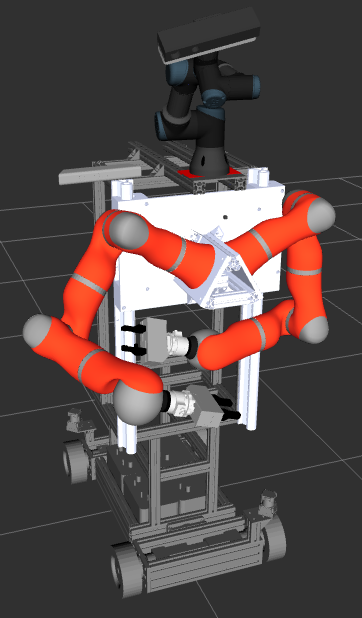
\includegraphics[width=0.3\linewidth]{boxy/visual.png}}
	\end{subfigure}
	~
	\begin{subfigure}[][Collision Model]
		{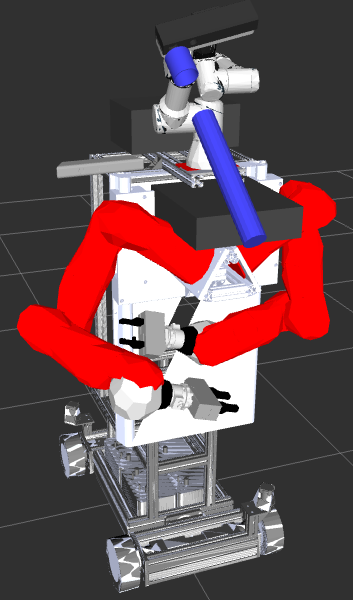
\includegraphics[width=0.3\linewidth]{boxy/collision.png}}
	\end{subfigure}
	\vspace{-15pt}
	\caption{Models of Boxy used by MoveIt!}
	\vspace{-10pt}
	\label{fig:models}
\end{figure}

The \textit{visualization model} is used by RViz (section \ref{subsec:rviz}) to visualize the robot in the computer. This model is normally as close as possible to the real robot, that means that the geometry tends to be complex and the files containing it are heavy. We use this model for visualizing the planned trajectory before executing it, or for visualizing the current state of the robot.

The \textit{collision model} of Boxy contains simplified geometry of the robot, it is usually slightly bigger than the real robot for security reasons. The collision model is the one MoveIt! uses while planning to check for collisions. Since the collision check is done for every pose in the trajectory and for every part in the model, it is convenient to have simplified geometry to speed up the calculations. The geometry of a model is represented in a mesh by triangles, a simplified model has fewer triangles than the one used for visualization. For example, the second link of the UR3 in the visualization model has 39702 triangles, and the collision model has only 849 triangles, that is 47 times less than the original model.

\subsection{RViz}
\label{subsec:rviz}

RViz is a 3D visualization tool for ROS. RViz displays the sensor data and the robot's state information taken from ROS. Using RViz we can visualize the current state of the robot (figure \ref{fig:rviz}), simulate trajectories, and display information from the sensors, such as 3D point-clouds from the Kinect.

\begin{figure}[H]
	\centering
	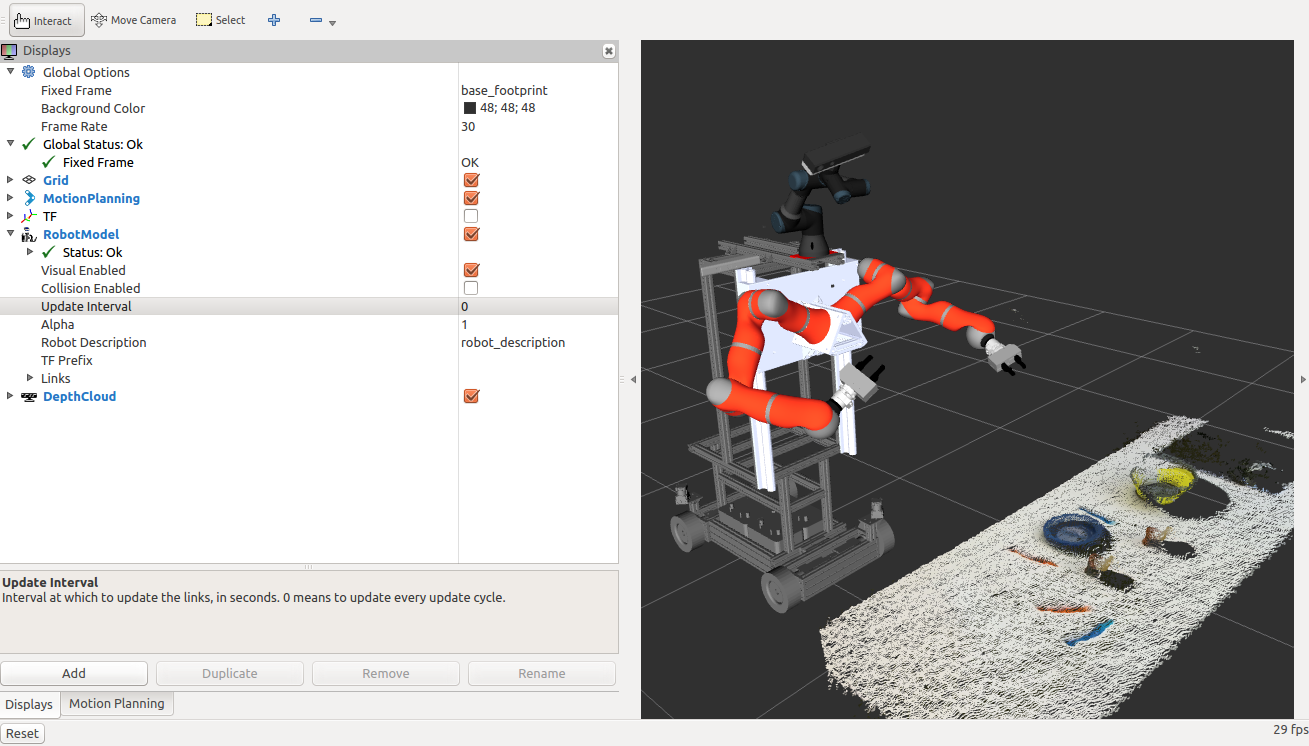
\includegraphics[width=0.85\linewidth]{boxy/rviz.png}
	\vspace{-10pt}
	\caption{RViz visualization of Boxy.}
	\vspace{-15pt}
	\label{fig:rviz}
\end{figure}

RViz uses a \textit{fixed frame} as a static reference for the visualization, the default frame is  \texttt{$\backslash$world}. All the information that RViz receives is displayed with respect to this frame, including: robot's current state, location of objects in the environment, and data from sensors.

\subsection{Giskard}

\subsection{Chili markers}